\documentclass[12pt]{article}

\usepackage[utf8]{inputenc}
\usepackage[brazil]{babel}
\usepackage[a4paper,left=3cm, right=2cm,top=2.5cm, bottom=2.5cm]{geometry}
\usepackage{amsmath}
\usepackage{graphicx}
\usepackage{float}
\usepackage{multirow}
\usepackage{authblk}
\usepackage{fancyhdr}
\usepackage{xcolor}
\usepackage{cite}


\title{\textbf{ENG1456 - Algoritmos Genéticos - Trabalho 2}}
\author{\textbf{Aluno: Matheus Carneiro Nogueira - 1810764}}
\affil{}
\author{\textbf{Professora: Karla Figueiredo}}
\affil{}
\pagestyle{fancy}
\fancyhf{}
\lhead{{\small \textcolor{gray}{PUC-Rio ENG1456}}}
\renewcommand{\headrulewidth}{0pt}
\date{}
\renewcommand{\footrulewidth}{0pt}
\fancyfoot[C]{\thepage}

\begin{document}
	\maketitle
	%\tableofcontents
	
	
	\begin{abstract}
		Este documento consiste no relatório do trabalho 2 do módulo de Algoritmos Genéticos da disciplina ENG1456 da PUC-Rio. O objetivo deste trabalho é estudar diferentes modelos de Algoritmos Genéticos para a tentativa de otimização da função Rastrigin. Foi utilizada a biblioteca geneticalgorithm2 para Python. Tudo que foi produzido para a realização deste trabalho encontra-se no repositório \textit{https://github.com/MathNog/Trabalhos\_ICA}, que será tornado público assim que o prazo para entrega deste trabalho se encerrar, com o intuito de evitar consultas indevidas e colas.
	\end{abstract}
	
	\section{Apresentação do Problema e comentários iniciais}
	
	O objetivo é avaliar e testar todos os parâmetros do Algoritmo Genético para encontrar a função de mínimo para o problema no menor tempo possível, ou seja, com a menor quantidade de gerações. O problema a ser minimizado é a função Rastrigin, definida por:
	\begin{equation*}
		f(x)=A_n+\sum_{i=1}^{n}[x_i^2-Acos(2\pi x_i)]
	\end{equation*}
	
	\begin{figure}[H]
		\centering
		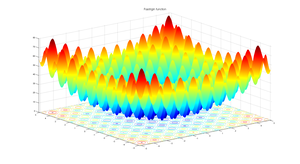
\includegraphics[width=0.9\linewidth]{Imagens/Rastrigin_function}
		\caption{Plot da função Rastrigin}
		\label{fig:rastriginfunction}
	\end{figure}
	
	Em cada seção desse relatório será variado algum parâmetro do algoritmo genético com o intuito de melhorar a minimização da função Rastrigin, com exceção da próxima seção que apresentará os resultados para os parâmetros iniciais padrões da biblioteca. Para visualizar e comparar resultados, serão fornecidas tabelas com os valores adotados para os parâmetros e imagens dos gráficos gerados pelo código.
	
	Os parâmetros que serão variados são \textit{max\_num\_iterarion}, \textit{population\_size}, \textit{mutation\_probability}, \textit{elit\_ratio}, \textit{crossover\_probability}, \textit{parents\_portion} e \textit{crossover\_type}. Sempre será variado um parâmetro por vez, mantendo os demais iguais ao GA inicial. Isso será feito para avaliar o impacto de cada parâmetro na qualidade do GA. Ao final, será executado um GA com os melhores valores para cada parâmetro variado.
	
	Serão sempre realizados 5 experimentos para cada configuração de GA e a análise será realizada com base nos resultamos médios de cada configuração.
	
	\section{GA com parâmetros iniciais dados}
	
	Os parâmetros utilizados no GA são:
	\begin{table}[H]
		\centering
		\begin{tabular}{|l|l|l|l|}
			\hline
			max\_num\_iterarion    & population\_size & mutation\_probability & elit\_ratio \\ \hline
			100                   & 100               & 0.1                     & 0.01           \\ \hline
			crossover\_probability & parents\_portion & crossover\_type       &             \\ \hline
			0.5                     & 0.3                & Uniform                     &             \\ \hline
		\end{tabular}
	\end{table}
	
	Para evitar repetição desnecessária, os gráficos que exibem os resultados do GA com parâmetros default serão exibidos apenas nesta seção. Nas demais seções apenas serão feitas referências a essas imagens com o intuito de realizar comparações na qualidade do algoritmo com os diferentes valores de parâmetros. 
	
	\begin{figure}[H]
		\centering
		\includegraphics[width=0.5\linewidth]{Imagens/graficoInicial}
		\caption{Gráfico do GA com parâmetros default}
		\label{fig:graficoinicial}
	\end{figure}
	\begin{figure}[H]
		\centering
		\includegraphics[width=0.5\linewidth]{Imagens/boxplotInicial}
		\caption{Boxplot do GA com parâmetros default}
		\label{fig:boxplotinicial}
	\end{figure}
	
	
	\section{Variação de max\_num\_iterarion} 
	
	Esse parâmetro define por quanto tempo nosso algoritmo ficará executando, o que, em outras palavras, significa a quantidade máxima de gerações. É importante que esse valor não seja pequeno demais para que a solução possua tempo para evoluir até uma solução razoável. Por outro lado, um valor alto pode ser desnecessário caso o algoritmo convirja para algum valor ótimo em menos gerações que o número máximo.
	
	\begin{table}[H]
		\centering
		\begin{tabular}{|l|l|l|l|l|}
			\hline
			\multicolumn{4}{|l|}{Número máximo de gerações}& Padrão \\ \hline
			10   & 50    & 200    & 500   & 100 \\ \hline
		\end{tabular}
	\end{table}
	
	
	\begin{figure}[H]
		\centering
		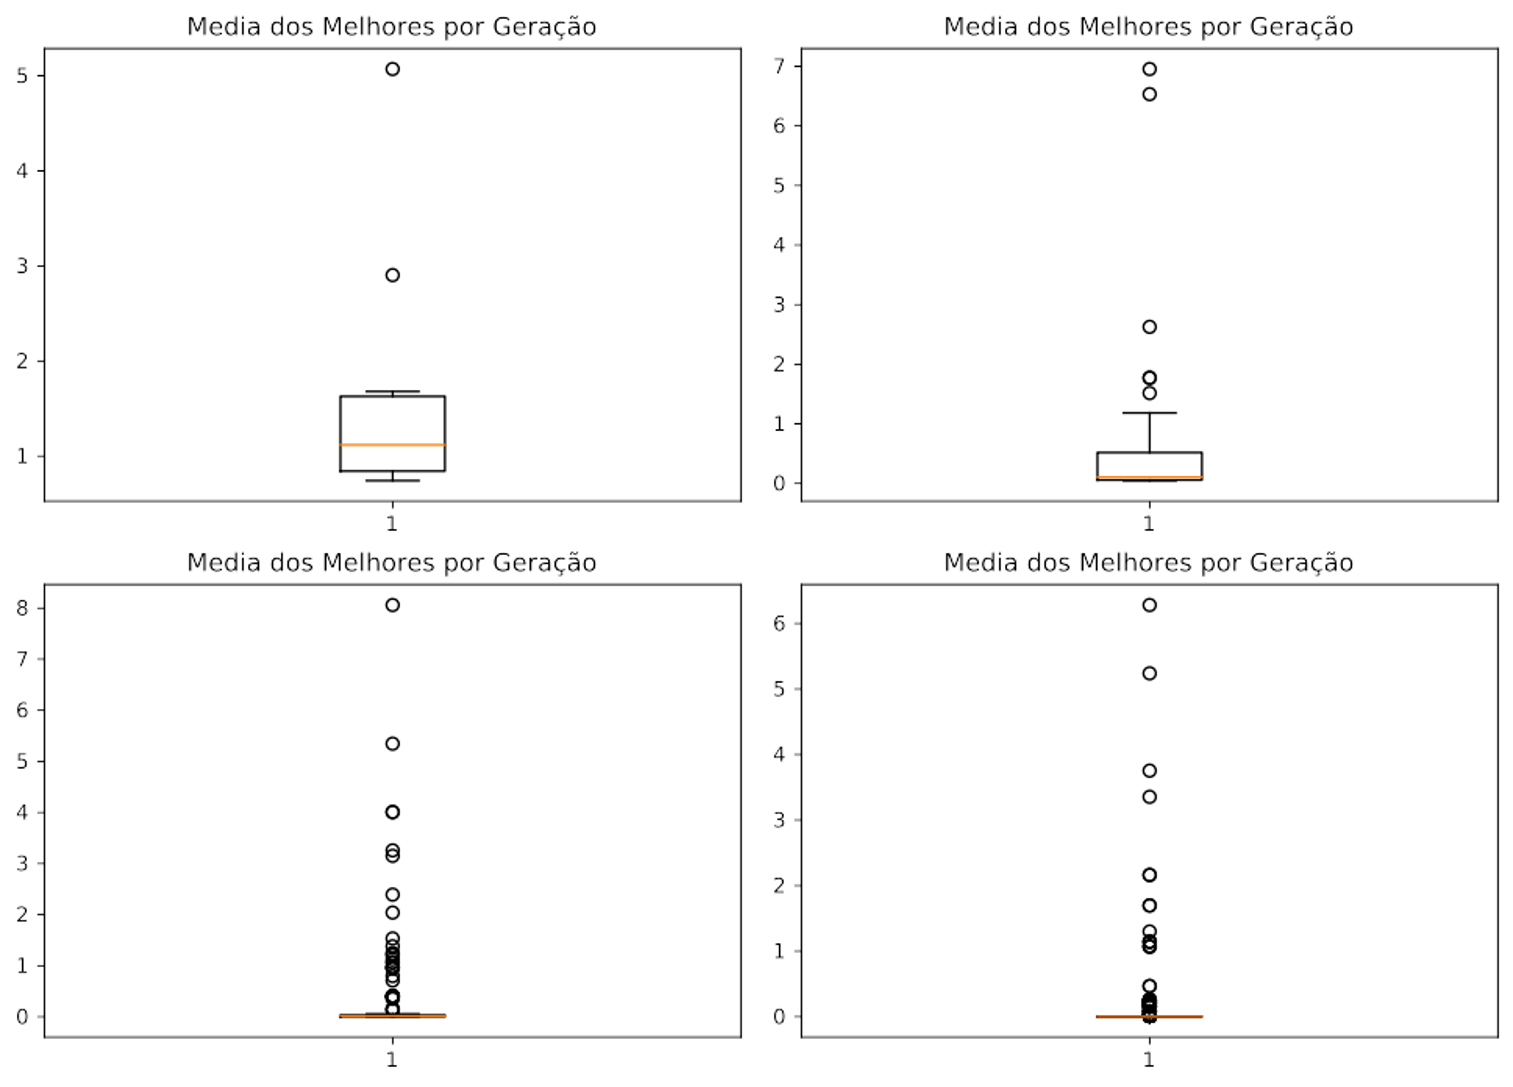
\includegraphics[width=0.9\linewidth]{Imagens/maxnumiteration/boxplotMaxNumIt}
		\caption{Boxplots variação max\_num\_iterarions}
		\label{fig:boxplotmaxnumit}
	\end{figure}
	\begin{figure}[H]
		\centering
		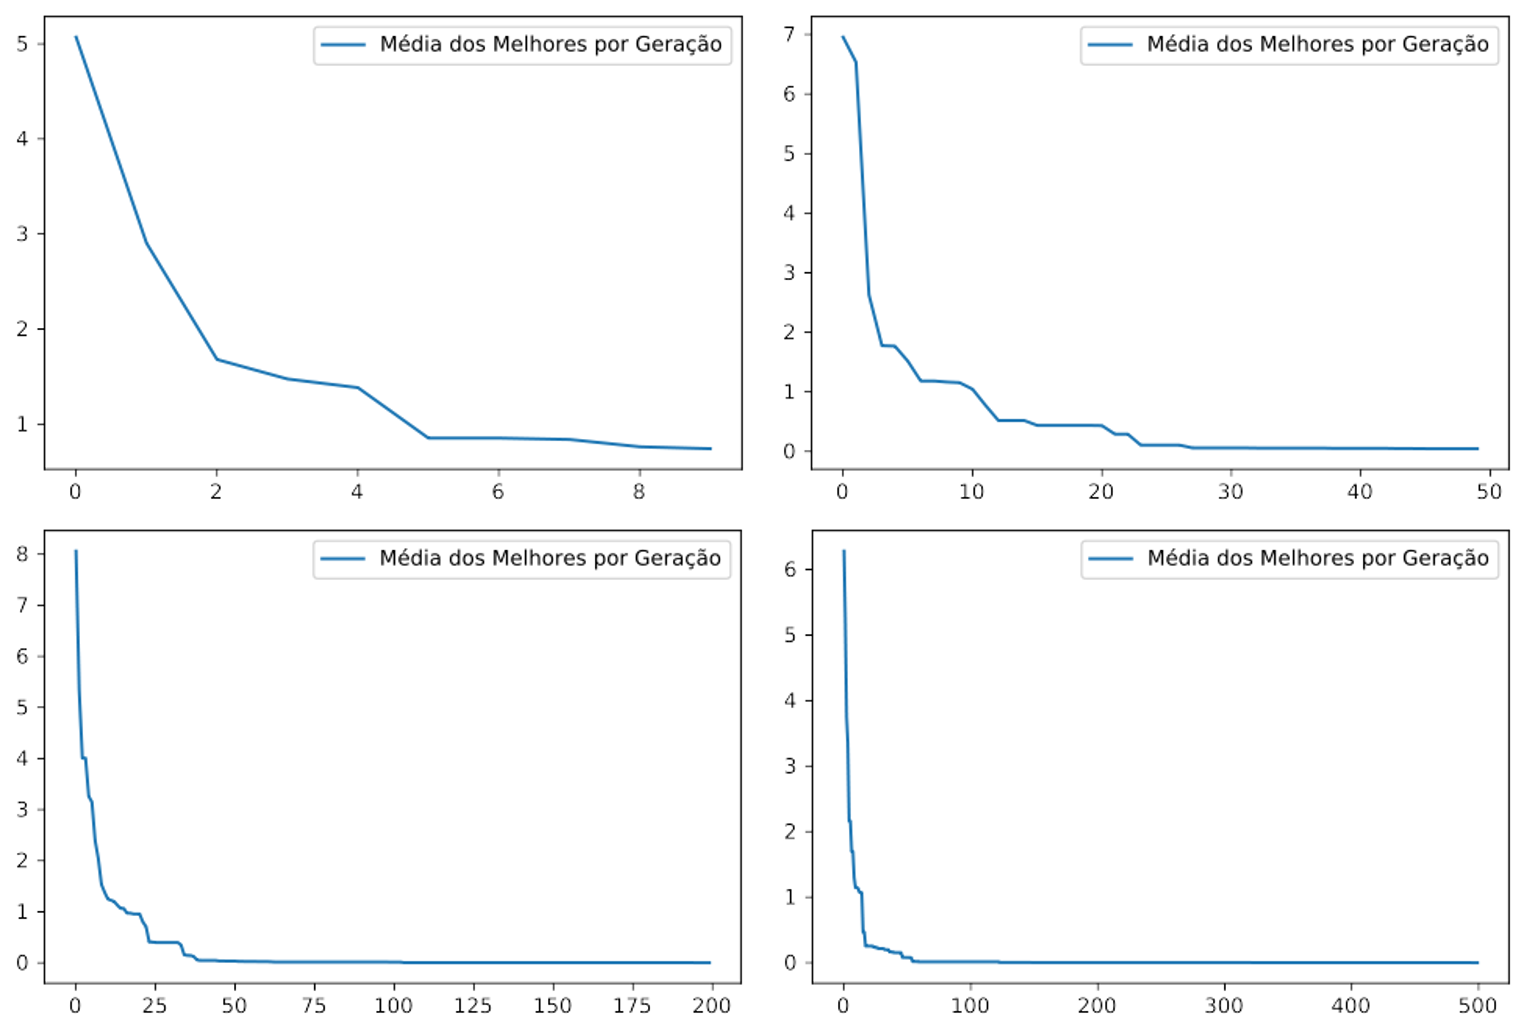
\includegraphics[width=0.9\linewidth]{Imagens/maxnumiteration/graficoMaxNumIt}
		\caption{Gráfico variação max\_num\_iterarions}
		\label{fig:graficomaxnumit}
	\end{figure}
	
	Ao analisar a figura \ref{fig:graficomaxnumit}, podemos chegar à seguinte conclusão: 10 gerações parece ser um número pequeno demais,  haja vista o fato da média dos melhores ser diferente de zero até, praticamente, o final das iterações. Por outro lado, valores a partir de 200 parecem ser desnecessariamente grandes, uma vez que muito antes do fim da execução do algoritmo a média dos melhores indivíduos já converge e fica parada em (ou muito pŕoximo de) zero.
	
	Partindo da figura \ref{fig:boxplotmaxnumit}, podemos perceber que para os valores de 200 e 500 há uma maior concentração de indivíduos em valores próximos de 0, o que faz sentido ao comparar com a figura \ref{fig:graficomaxnumit}. Por outro lado, ao analisar o boxplot de \textit{max\_num\_iteration=10}, notamos que 75\% dos dados, o que corresponde a todos os quartis exceto o primeiro, estão acima de 1 e apenas 25\% abaixo de 1, o que revela que poucos indivíduos possuem avaliação boa, próxima de zero.
	
	Sendo assim, podemos concluir que o valor ótimo para essa variável está próximo do 100 ou 200. Na última seção rodaremos um GA com \textit{max\_num\_iteration=150}.
	
	
	\section{Variação de population\_size}
	
	O tamanho da população é a quantidade de indivíduos em cada geração. Podemos pensar na variação desse parâmetro como uma intensificação de busca paralela. Quanto mais indivíduos na população, maior o paralelismo da busca pela solução ótima, embora exija maior capacidade computacional. Uma população pequena demais levaria muito tempo para alcançar um valor de aptidão específico enquanto que uma população maior o alcançaria mais rápido.
	
	\begin{table}[H]
		\centering
		\begin{tabular}{|l|l|l|l|l|}
			\hline
			\multicolumn{4}{|l|}{Tamanho da População}& Padrão \\ \hline
			10   & 50    & 200    & 500   & 100 \\ \hline
		\end{tabular}
	\end{table}
	
	\begin{figure}[H]
		\centering
		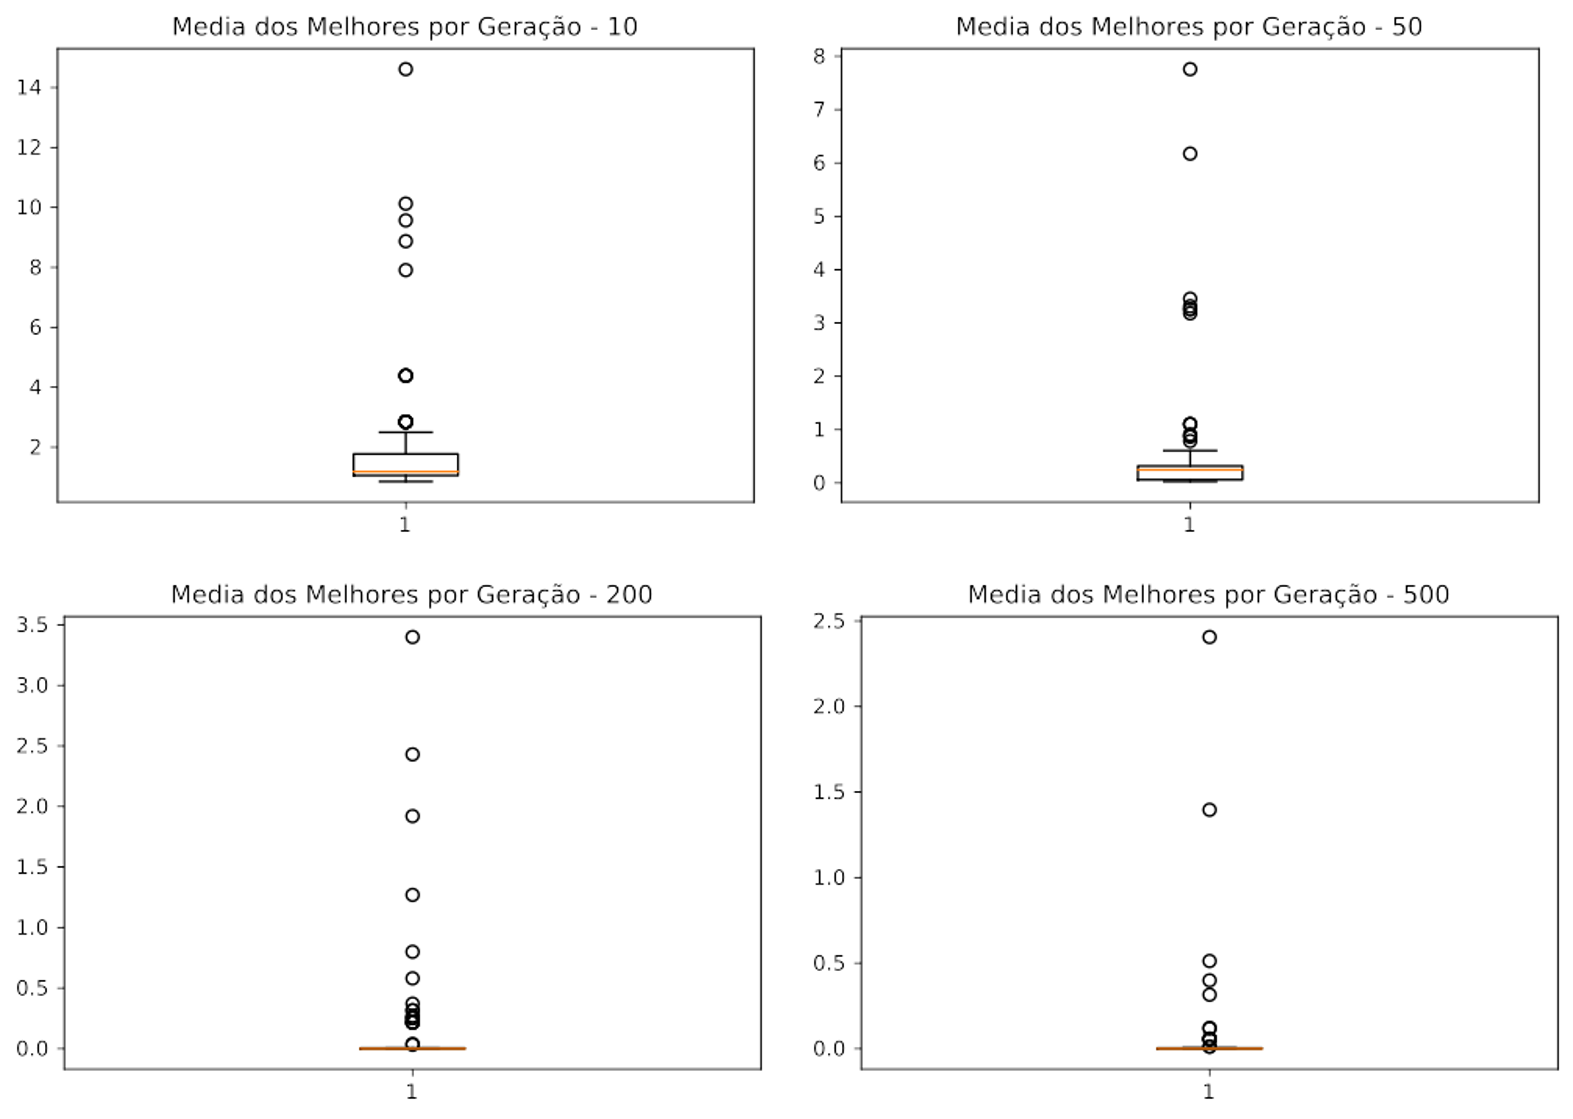
\includegraphics[width=0.9\linewidth]{Imagens/populationSize/boxplotPopSize}
		\caption{Boxplots variação population\_size}
		\label{fig:boxplotpopsize}
	\end{figure}
	\begin{figure}[H]
		\centering
		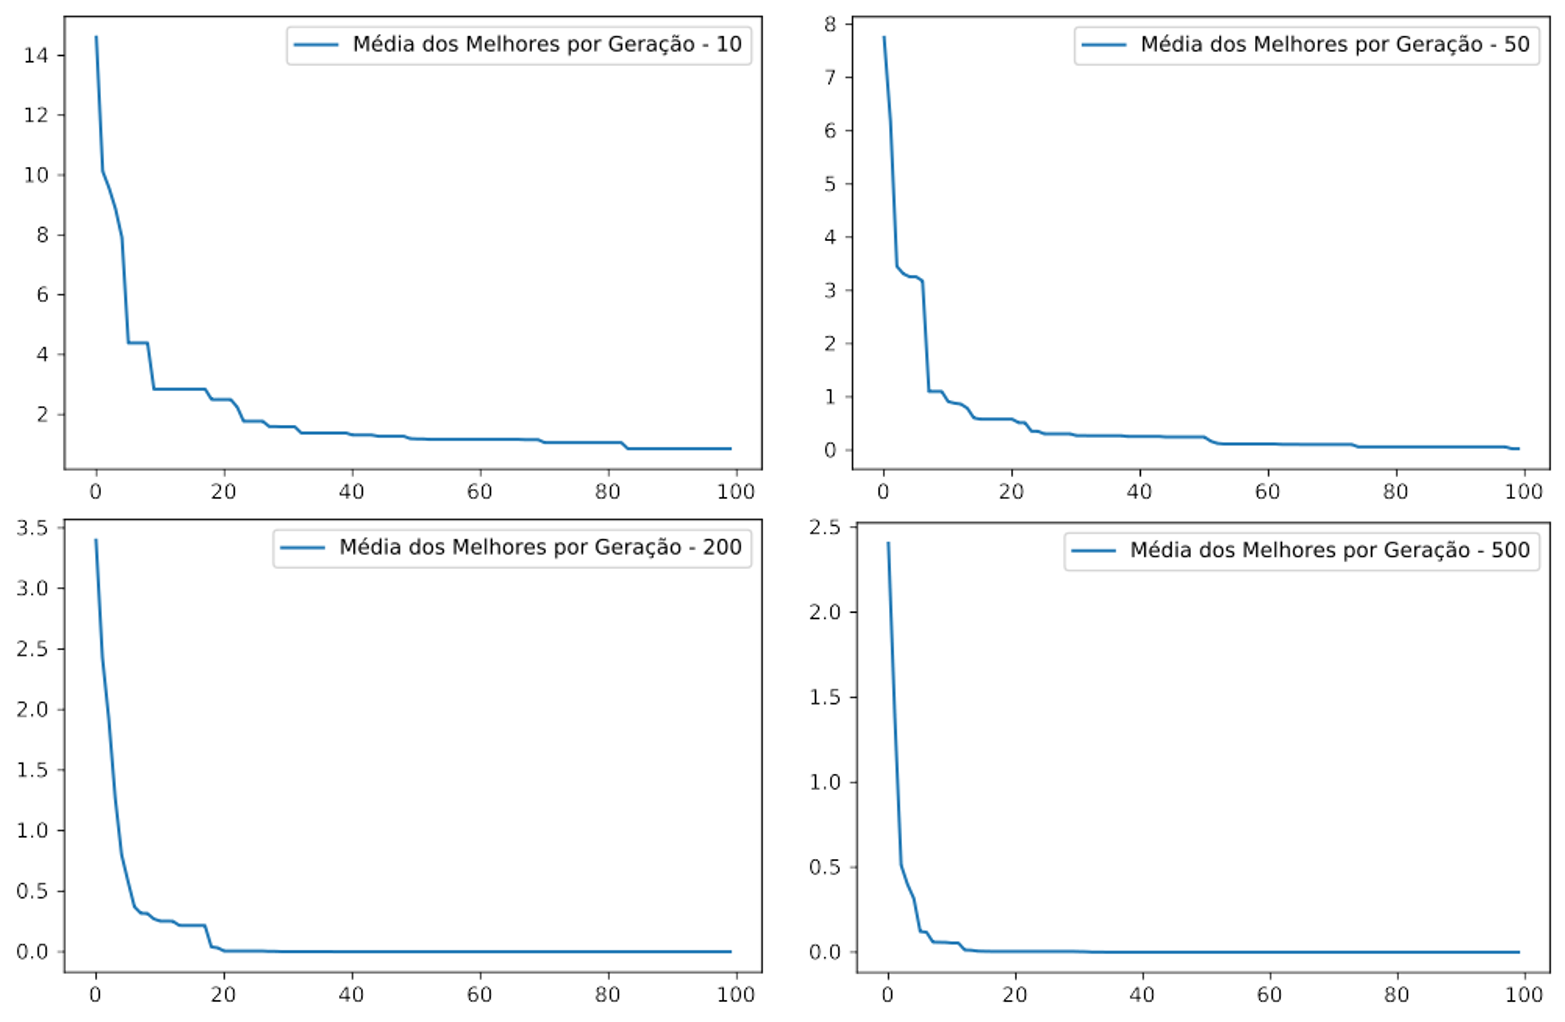
\includegraphics[width=0.9\linewidth]{Imagens/populationSize/graficoPopSize}
		\caption{Gráficos variação population\_size}
		\label{fig:graficopopsize}
	\end{figure}
	
	Com base na análise de ambas as figuras \ref{fig:boxplotpopsize} e \ref{fig:graficopopsize}, podemos perceber que para valores maiores desse parâmetro a convergência para a média dos melhores indivíduos para valores próximos de zero é maior que para valores pequenos. Percebemos isso tanto pela rápida queda dos gráficos inferiores da figura \ref{fig:graficopopsize} quanto pelo fato dos 3 primeiros quartis (75\%) dos melhores indivíduos estar abaixo de 1 nos boxplots inferiores da figura \ref{fig:boxplotpopsize}. Isso confirma o que era suposto em relação a variação do tamanho da população.
	
	Além disso, podemos perceber que o perfil do gráfico da média dos melhores indivíduos para populações de 200 e 500 é muito similar, não justificando, portanto, aumentar o gasto computacional com uma população tão grande.
	
	Sendo assim, podemos supor que o valor ótimo para o tamanho da população para este problema é próximo de 200. Dito isso, na útima seção, utilizaremos \textit{population\_size=250}.
	
	\section{Variação de mutation\_probability}
	
	Variar a taxa de mutação é variar a aleatoriedade do processo de evolução do GA, uma vez que uma mutação é uma alteração aleatória em alguns dos genes, ou indivíduos, do algoritmo. Valores de mutação muito altos geram processos muito aleatórios que podem frear a evolução da minimização, embora a existência de, pelo menos, uma taxa pequena seja importante para aumentar as chances do algoritmo ser capaz de gerar todas as combinações de indivíduos.
	
	A tabela abaixo exibe os diferentes valores de taxa de mutação testados:
	
	\begin{table}[H]
		\centering
		\begin{tabular}{|l|l|l|l|l|}
			\hline
			\multicolumn{4}{|l|}{Taxa de Mutação} & Padrão \\ \hline
			0.001    & 0.3    & 0.7    & 1.0    & 0.1    \\ \hline
		\end{tabular}
	\end{table}
	
	\begin{figure}[H]
		\centering
		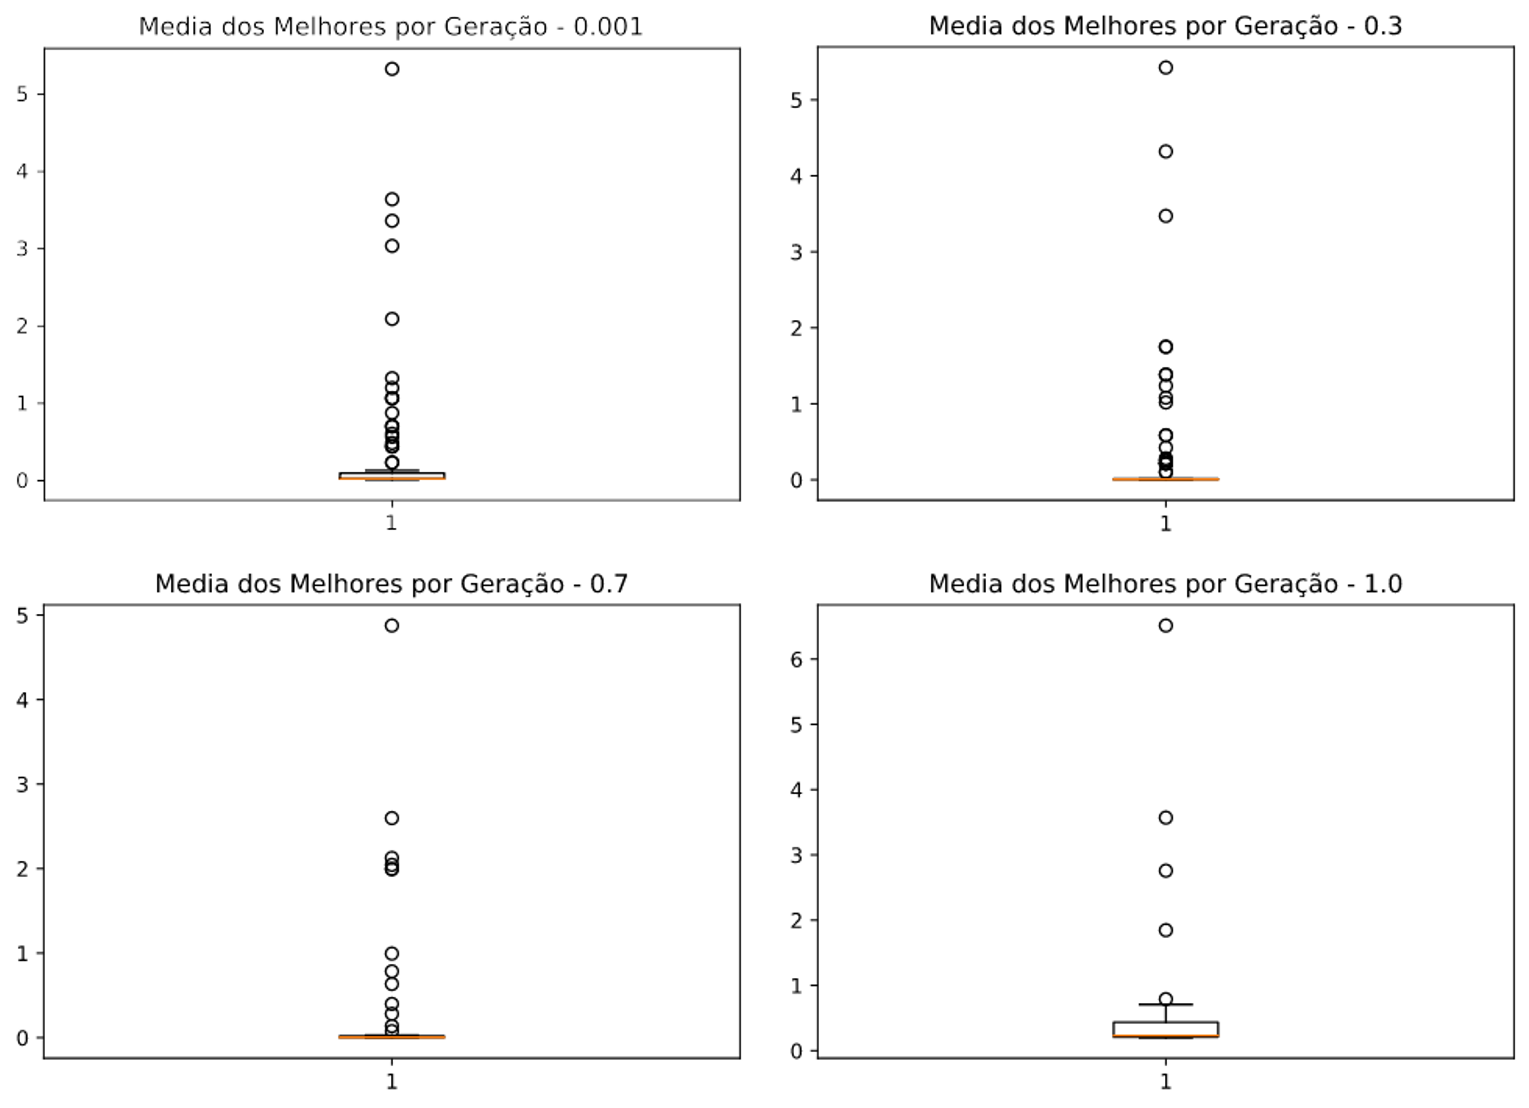
\includegraphics[width=0.9\linewidth]{Imagens/mutacao/boxplotMutacao}
		\caption{Boxplots variação mutation\_probability}
		\label{fig:boxplotmutacao}
	\end{figure}
	\begin{figure}[H]
		\centering
		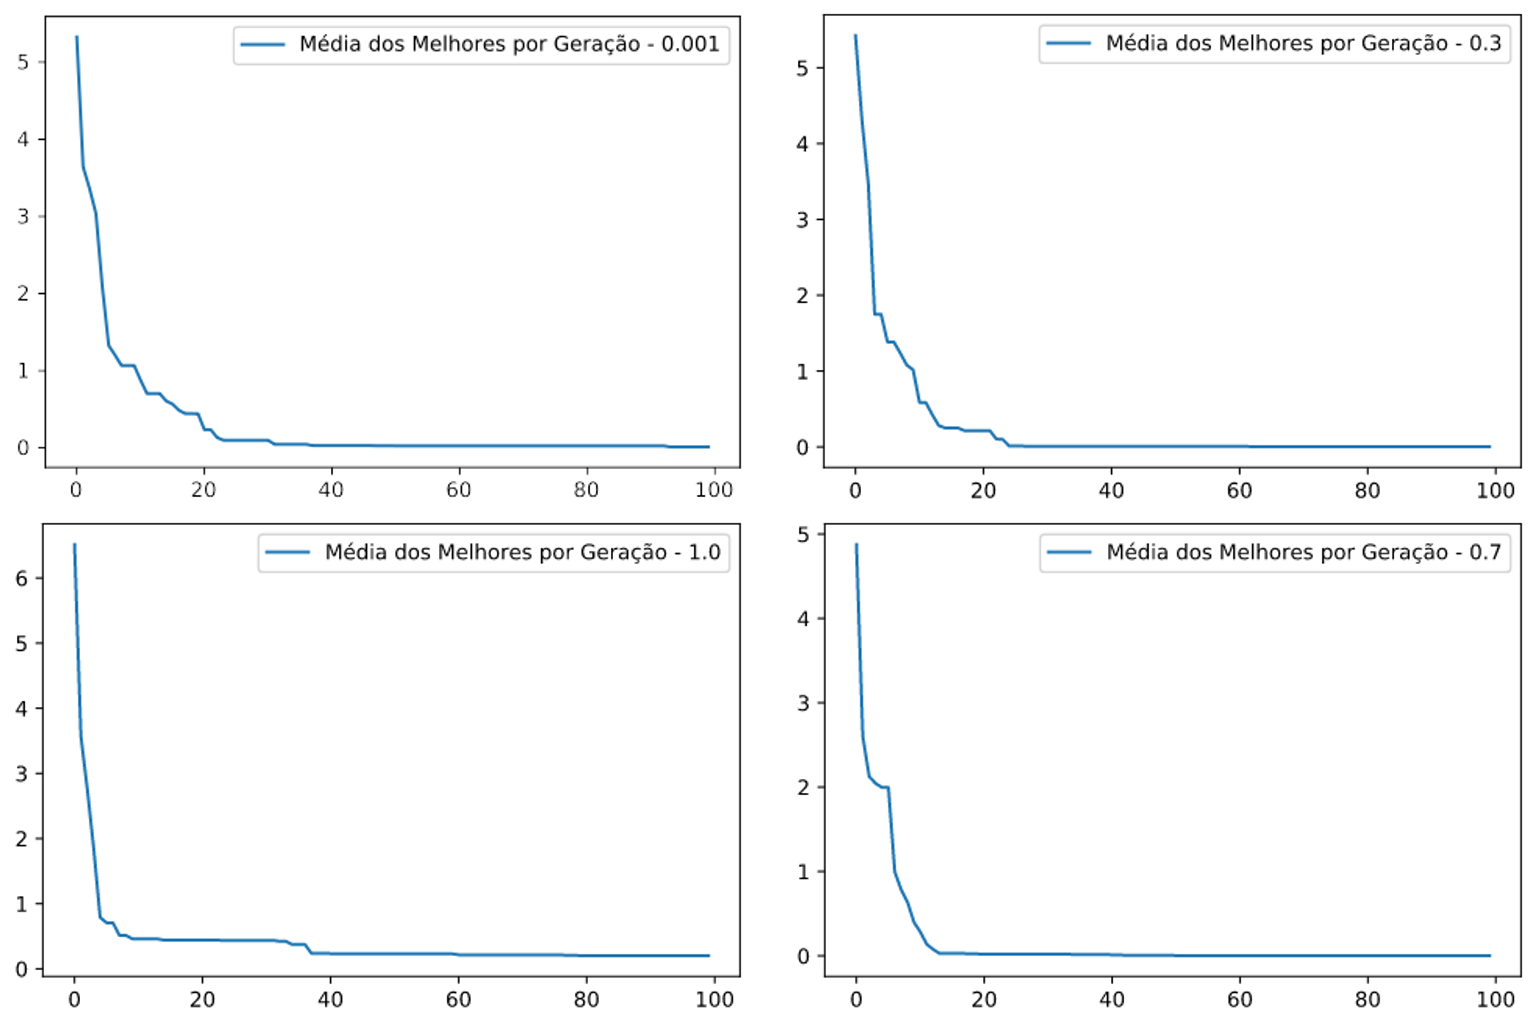
\includegraphics[width=0.9\linewidth]{Imagens/mutacao/graficoMutacao}
		\caption{Gŕaficos variação mutation\_probability}
		\label{fig:graficomutacao}
	\end{figure}
	
	Ao analisar os gráficos da figura \ref{fig:graficomutacao} houve uma surpresa. Imaginava que o caso em que em 100\% das vezes ocorresse mutação o desempenho do GA apresentar-se-ai muito pior, devido ao maior grau de aleatoriedade inserido na evolução do GA. No entanto, não é isso que percebemos. O que, talvez, explique isso seja o fato de também estarmos aplicando elitismo, garantindo que o melhor da geração seguinte nunca seja pior que o melhor da geração anterior. 
	
	Somado a isso, os boxplots para os valores de 0.001 e 0.3 são muito similares entre si e também quando comparados ao valor default, 0.1, o que nos indica que alterar a taxa de mutação implica, neste problema, em pouca alteração na qualidade do GA. Podemos reparar, também, que o boxplot para o valor 1 apresenta segundo, terceiro e quarto quartis maiores que os demais, o que indica uma piora na qualidade do GA.
	
	Resumindo, embora considere estranho o pouco impacto da variação da taxa de mutação, existe uma explicação razoável que explica esse fato. Sendo assim, um valor próximo do ótimo, dentre os valores utilizados, parece ser 0.3.
	
	\section{Variação de elit\_ratio}
	
	Esse parâmetro configura o elitismo do algoritmo genético, sendo a taxa em si a porcentagem dos melhores indivíduos que será mantida para a próxima geração. Como sabemos, o elitismo é importante para mantermos a curva de otimização monotônica, neste caso sempre decrescente haja vista o fato do problema ser uma minimização. Uma taxa zero significa não haver elitismo. Taxas muito altas freiam o processo uma vez que haverá poucos novos indivíduos sendo gerados a cada geração. Taxas pequenas demais, por sua vez, aumentam as chances de termos mais indivíduos piores do que melhores na próxima geração.
	
	A variação deste parâmetro é limitada pela porcentagem de pais a serem mantidos, de acordo com o parâmetro \textit{parents\_portion}. Sendo assim, conseguiremos testar apenas valores abaixo de $0.3$.
	
	A tabela abaixo exibe os diferentes valores de taxa de elitismo testados:
	
	\begin{table}[H]
		\centering
		\begin{tabular}{|l|l|l|l|}
			\hline
			\multicolumn{3}{|l|}{Taxa de Elitismo} & Padrão \\ \hline
			0.0    & 0.001    & 0.1    & 0.01    \\ \hline
		\end{tabular}
	\end{table}
	
	\begin{figure}[H]
		\centering
		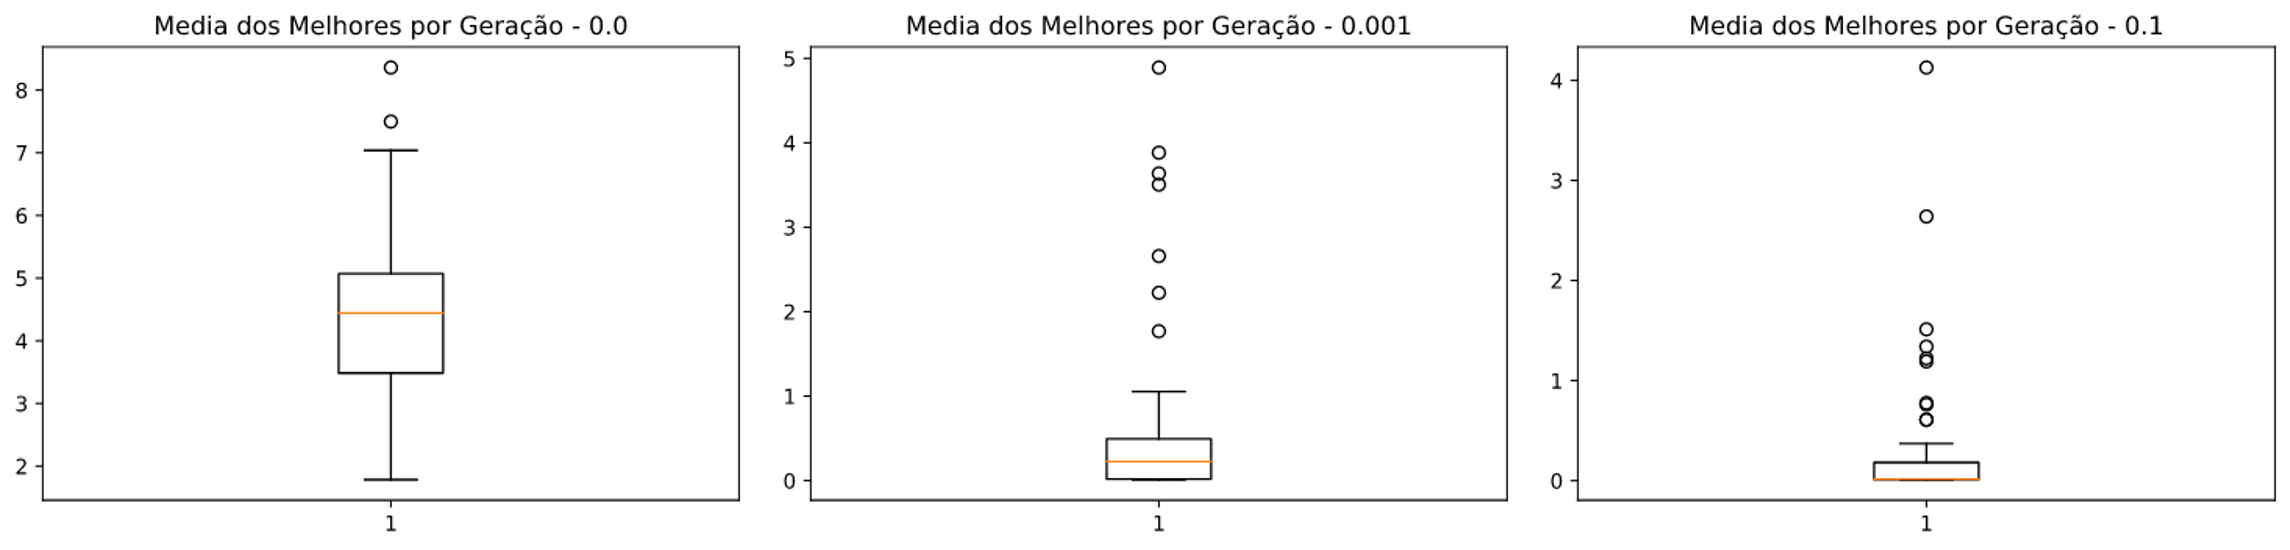
\includegraphics[width=0.9\linewidth]{Imagens/elitismo/boxplotElitismo}
		\caption{Boxplots variação elit\_ratio}
		\label{fig:boxplotelitismo}
	\end{figure}
	\begin{figure}[H]
		\centering
		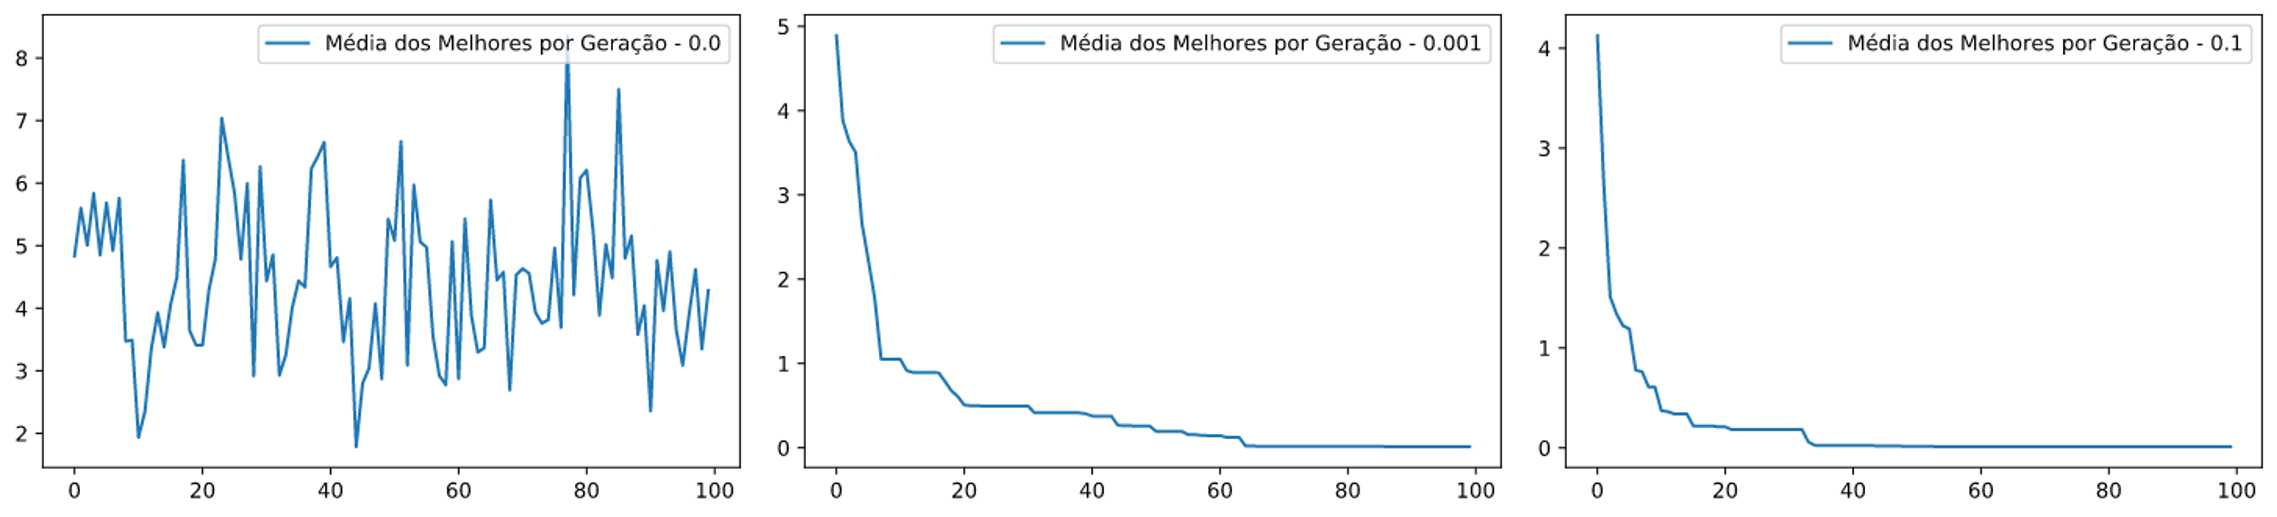
\includegraphics[width=0.9\linewidth]{Imagens/elitismo/graficoElitismo}
		\caption{Gráficos variação elit\_ratio}
		\label{fig:graficoelitismo}
	\end{figure}
	
	Ao analisar as duas figuras acima, um fato é facilmente percebido: GA sem elitismo é ruim. Não é possível observar nenhuma tendência de convergência para o valor ótimo, visto que a média dos melhores por geração é, praticamente, estacionária e muito volátil. O boxplot para esse caso exibe o mesmo, uma vez que o valor mínimo exibido é 2. 
	
	Como comentado acima, a variação deste parâmetro possui um limite superior forçado pela configuração da biblioteca. Sendo assim, uma faixa pequena de valores foi testada, além de todos serem menores ou igual a 0.1. Mesmo assim, percebemos que a taxa de 0.001 é razoavelmente pior que a de 0.1, uma vez que seu boxplot é mais disperso e seu gráfico possui, entre as gerações 10 e 60, uma queda mais suave do que o da taxa 0.1. Por fim, ao comparar esse resultado com o valor default, 0.01, percebe-se, também, pouca diferença, com melhores resultados para o valor 0.1.
	
	Conclui-se, portanto, que valores próximos de 0.1 são os mais adequados para esse problema.
	
	
	\section{Variação de crossover\_probability}
	
	Variar a taxa de crossover significa variar a taxa com a qual o algoritmo gera novos descendentes a partir dos progenitores. Altas taxas de crossover aumentam a combinação de progenitores para a geração de filhos, enquanto baixas taxas fazem com que mais filhos sejam idênticos aos pais. Taxas altas demais não são interessantes por "embaralhar" demais os filhos, fazendo com que o perfil da evolução possa ser perdido. Por outro lado, taxas pequenas demais também não são interessantes por diminuir a variabilidade genética dos filhos, o que pode frear a evolução.
	
	A tabela abaixo exibe os diferentes valores de taxa de crossover testados:
	
	\begin{table}[H]
		\centering
		\begin{tabular}{|l|l|l|l|l|}
			\hline
			\multicolumn{3}{|l|}{Taxa de Crossover} & Padrão \\ \hline
			0.25    & 0.75    & 1   &0.5 \\ \hline
		\end{tabular}
	\end{table}
	
	\begin{figure}[H]
		\centering
		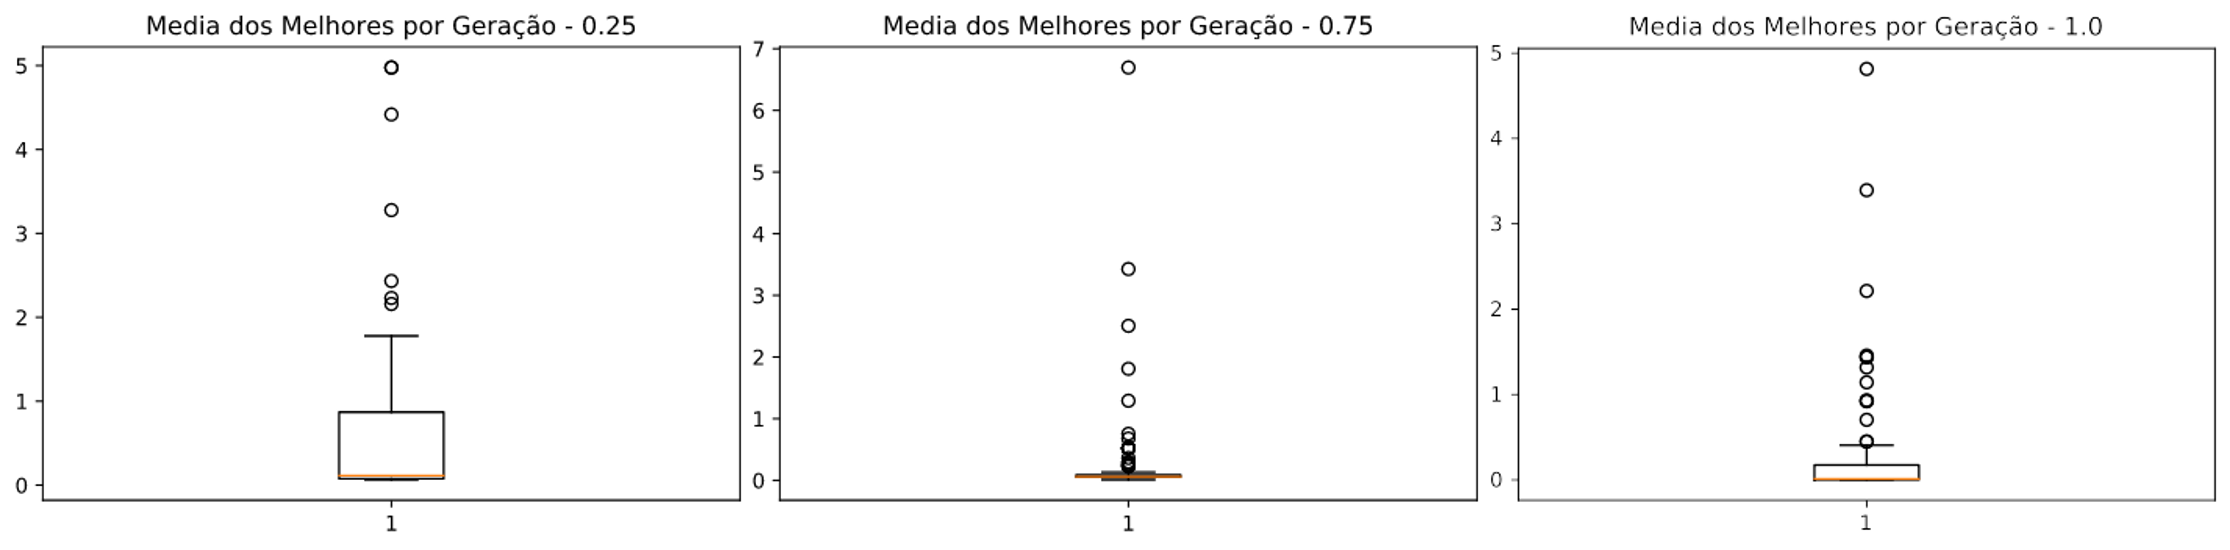
\includegraphics[width=0.9\linewidth]{Imagens/crossover/boxplotTaxaCross}
		\caption{Boxplot variação crossover\_probability}
		\label{fig:boxplottaxacross}
	\end{figure}
	\begin{figure}[H]
		\centering
		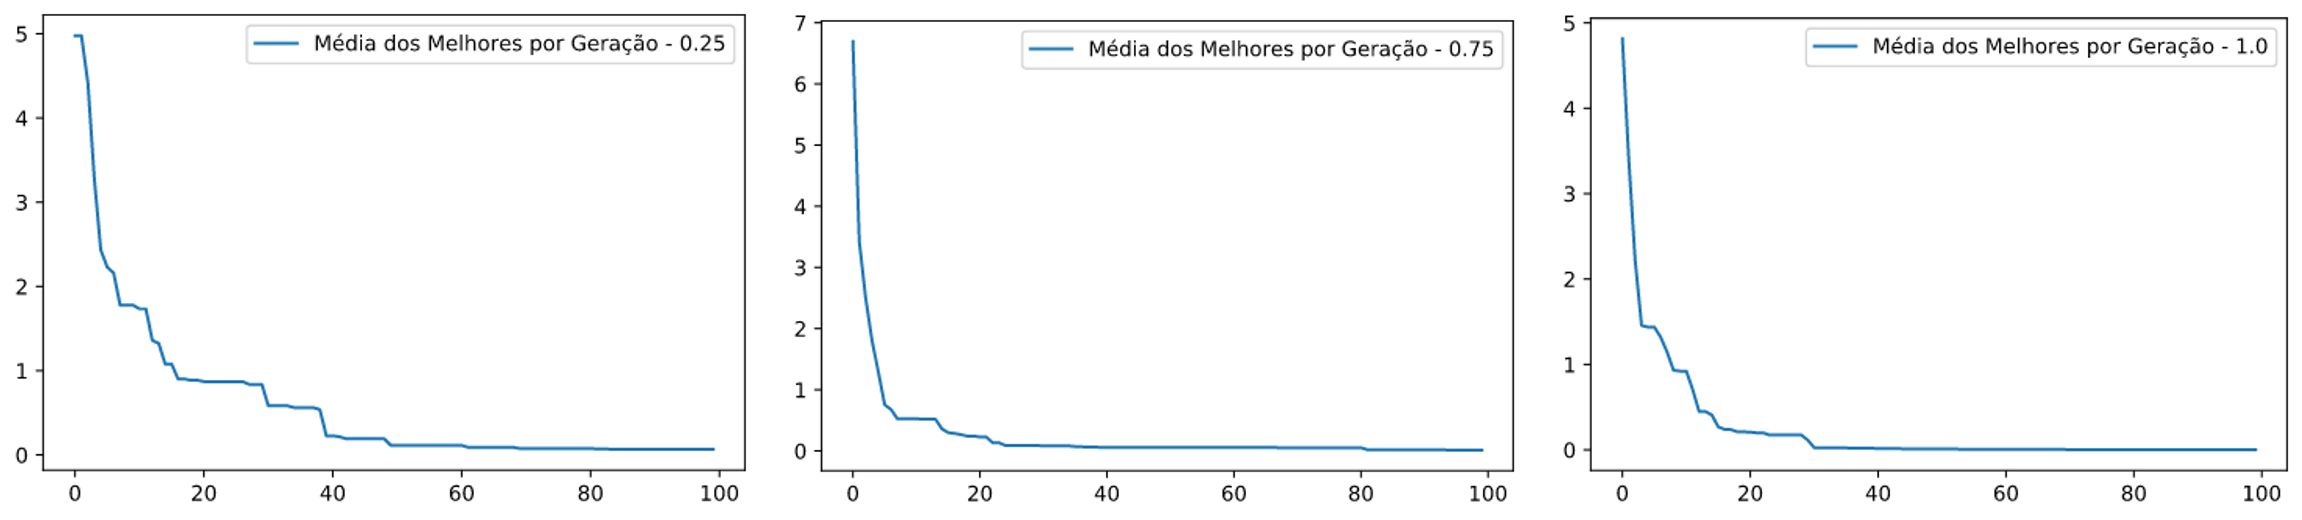
\includegraphics[width=0.9\linewidth]{Imagens/crossover/graficoTaxaCross}
		\caption{Gráficos variação crossover\_probability}
		\label{fig:graficotaxacross}
	\end{figure}
	
	Um primeiro comentário que deve ser feito é que a biblioteca utilizada não permite taxa de crosover igual a 0.
	
	Dito isso, ao analisar os 3 boxplots, nota-se rapidamente que o valor de 75\% apresenta o melhor resultado, uma vez que revela maior quantidade de indivíduos, 3 primeiros quartis,muito próximos de 0. Realizar crossover em 100\% das vezes não é vantajoso, assim como previsto na teoria. Isso é percebido pelo gráfico da figura \ref{fig:graficotaxacross} que mostra, entre as geraçoes 10 e 30, caráter decrescente mais suave que o apresentado pela taxa de 75\%. A razão disso já foi explicitada: "embaralhar" demais os progenitores dificulta a convergência para a solução ótima uma vez que adiciona aleatoriedade ao processo de evolução.
	
	Ao comparar com o valor default, 0.5, notamos pela análise de ambos os gráficos que o valor 0.75 ainda mostra-se mais adequado. Sendo assim, ele é o eleito como valor mais próximo do ótimo dentre os testados. 
	
	\section{Variação de parents\_portion}
	
	A definição desse parâmetro na documentação da biblioteca não é muito clara e se confunde com a definição de elit\_ratio. Suponho, com base no que entendi e discuti com a professora, que a porção de pais que o GA mantém não é, necessariamente, a melhor. Essa hipótese ganha força pelo fato de que a porcentagem \textit{parents\_portion} inclui, segundo a documentação, a porcentagem definida em \textit{elit\_ratio}. Dito isso, a análise do impacto deste parâmetro sozinho talvez não traga muitas informações interessantes. De todo modo, foram testados diferentes valores, assim como descrito na tabela abaixo:
	
	\begin{table}[H]
		\centering
		\begin{tabular}{|l|l|l|l|l|}
			\hline
			\multicolumn{4}{|l|}{Porcentagem de Pais mantidos} & Padrão \\ \hline
			0.02    & 0.1    & 0.7    & 1   &0.3 \\ \hline
		\end{tabular}
	\end{table}
	
	\begin{figure}[H]
		\centering
		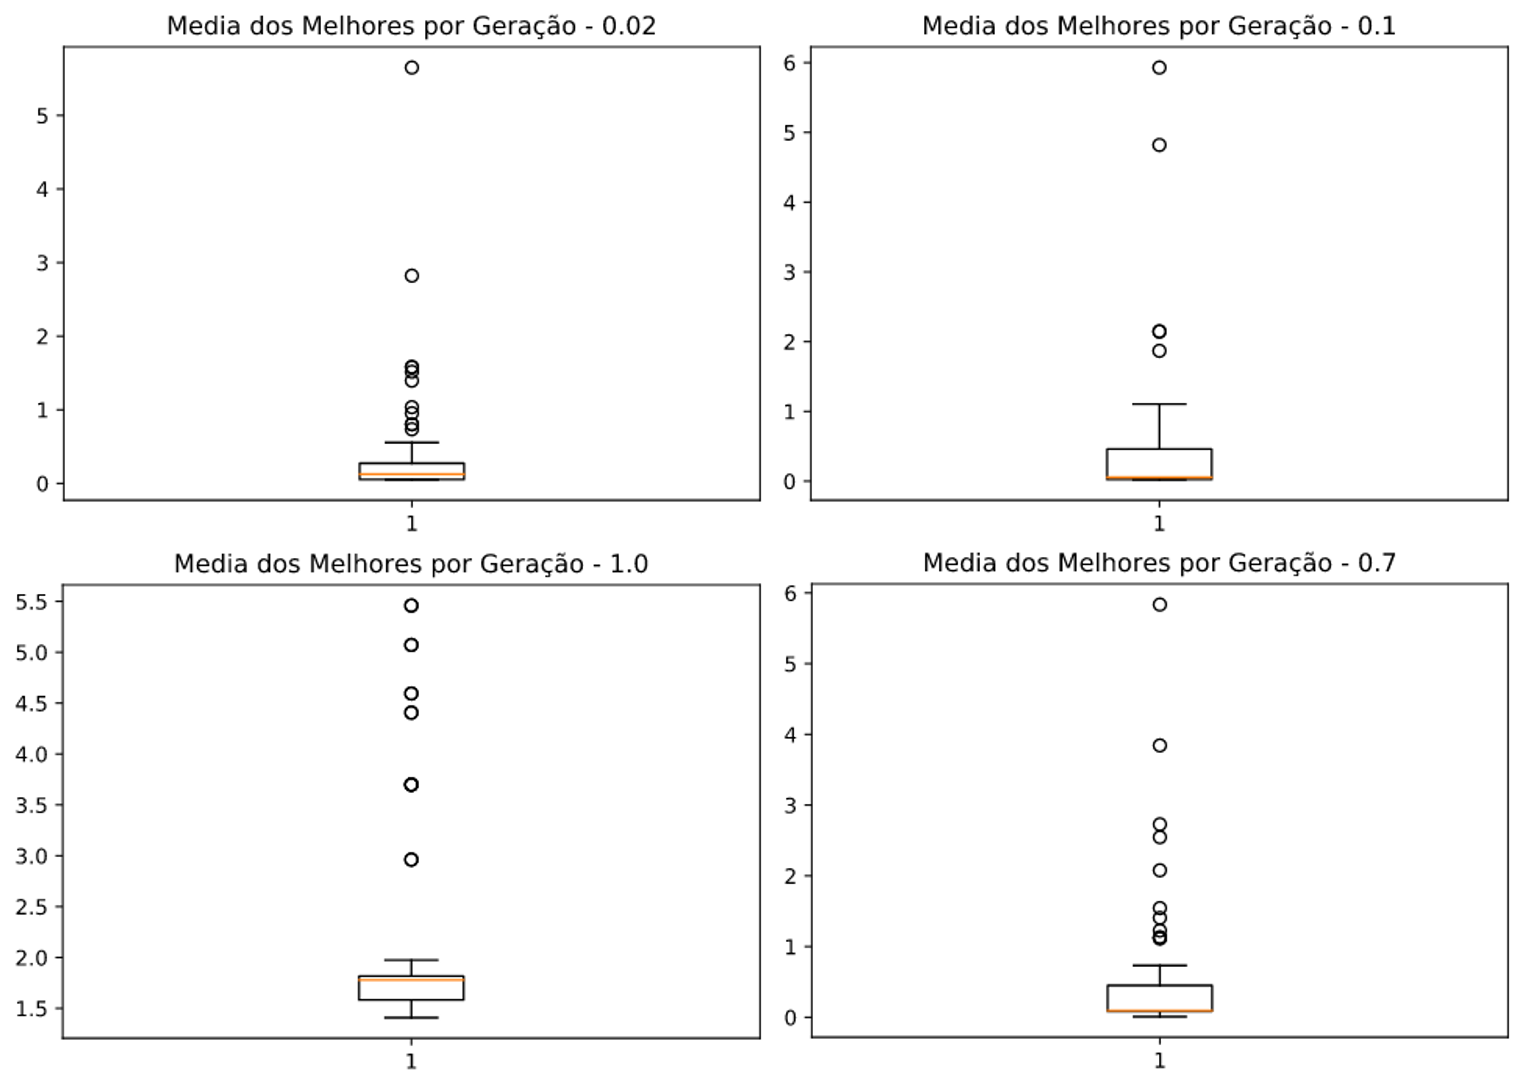
\includegraphics[width=0.9\linewidth]{Imagens/parentsPortion/boxplotParPor}
		\caption{Boxplots variação parents\_portion}
		\label{fig:boxplotparpor}
	\end{figure}
	\begin{figure}[H]
		\centering
		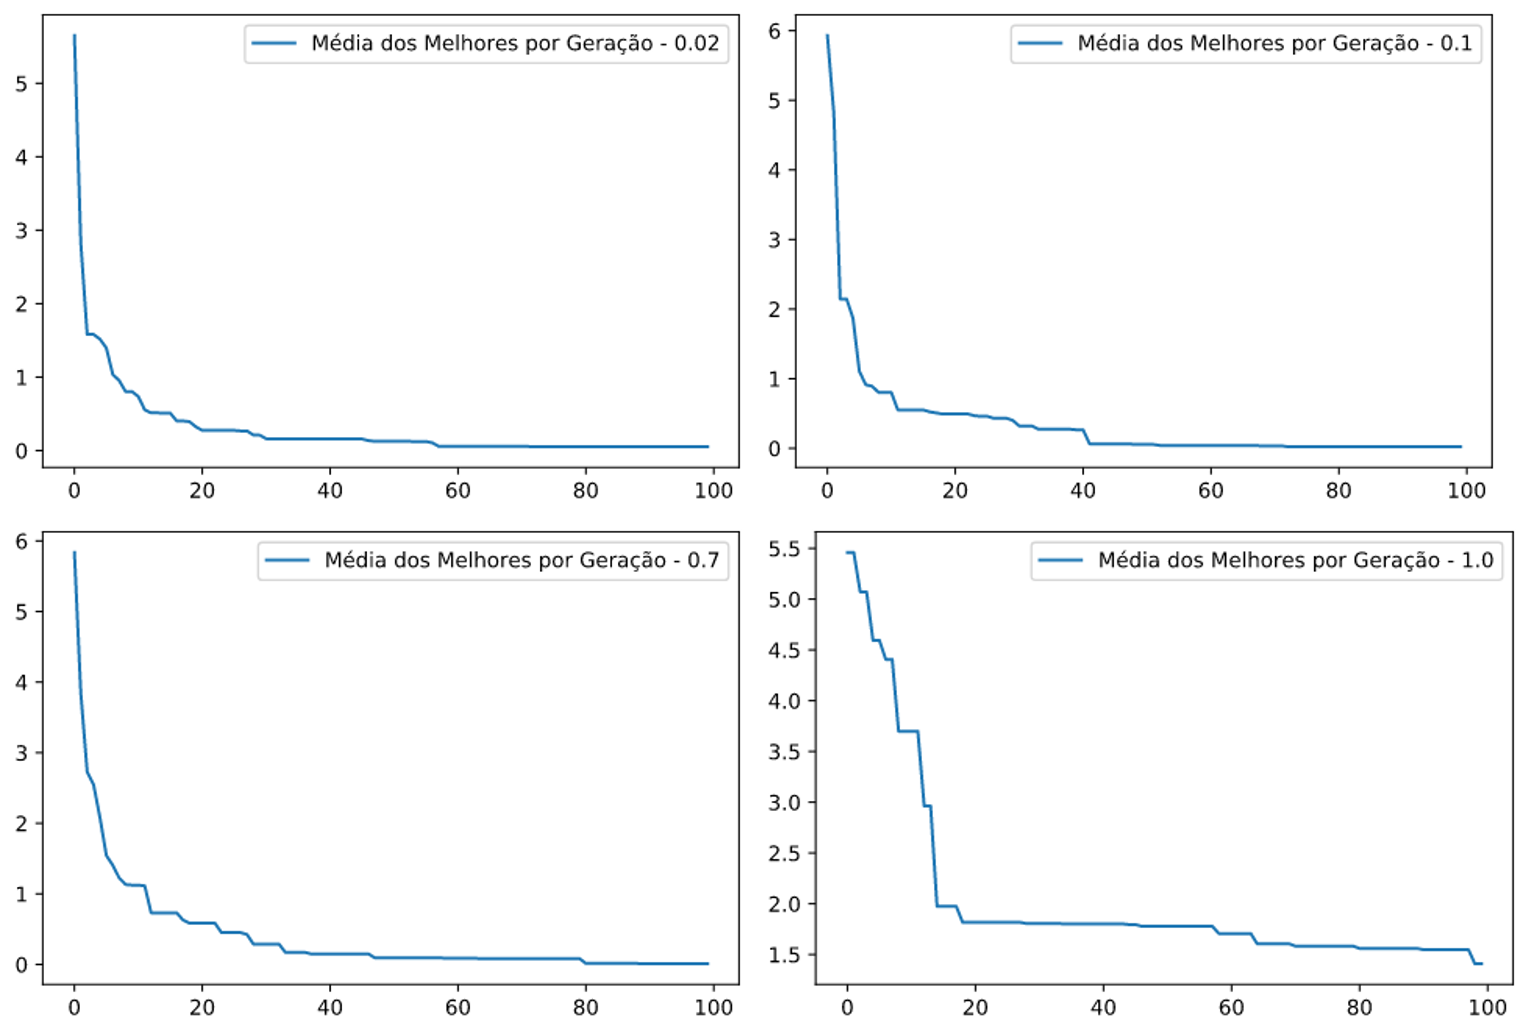
\includegraphics[width=0.9\linewidth]{Imagens/parentsPortion/graficoParPor}
		\caption{Gráficos variação parents\_portion}
		\label{fig:graficoparpor}
	\end{figure}
	
	Como discutido no parágrafo anterior, podemos perceber que a variação deste parâmetro não impactou muito na qualidade do GA. Isso se explica pelo fato de que manter mais ou menos pais para a geração seguinte, sem garantir que eles sejam os melhores pais, é indiferente e não colabora com a convergência para a minimização da função. Variar este parâmetro, portanto, sem variar a taxa de elitismo, é próximo do inútil. Além disso, pode-se notar que, mantendo o valor de elitismo fixo, valores pequenos de \textit{parents\_portion} parecem ser melhores. Isso faz sentido pois, como não estamos mantendo, necessariamente, os melhores pais é melhor manter poucos para a geração seguinte.
	
	Sendo assim, manteremos o valor default para a execução do GA da última seção.
	
	\section{Variação de crossover\_type}
	
	São três os tipos de crossover disponíveis: um ponto, dois pontos e uniforme. Enquanto os dois primeiros simplesmente escolhem, aleatoriamente, um ou dois pontos de corte do gene para cruzamento, o último utiliza um padrão, também aleatório, para comparar com os progenitores. Os dois últimos tipos, dois pontos e uniforme, são capazes de combinar todos os padrões dos progenitores, enquanto o de um ponto não.
	
	\begin{table}[H]
		\centering
		\begin{tabular}{|l|l|l|}
			\hline
			\multicolumn{2}{|l|}{Tipos de Crossover}&Padrão \\ \hline
			OnePoint    & TwoPoints    & Uniform    \\ \hline
		\end{tabular}
	\end{table}
	
	\begin{figure}[H]
		\centering
		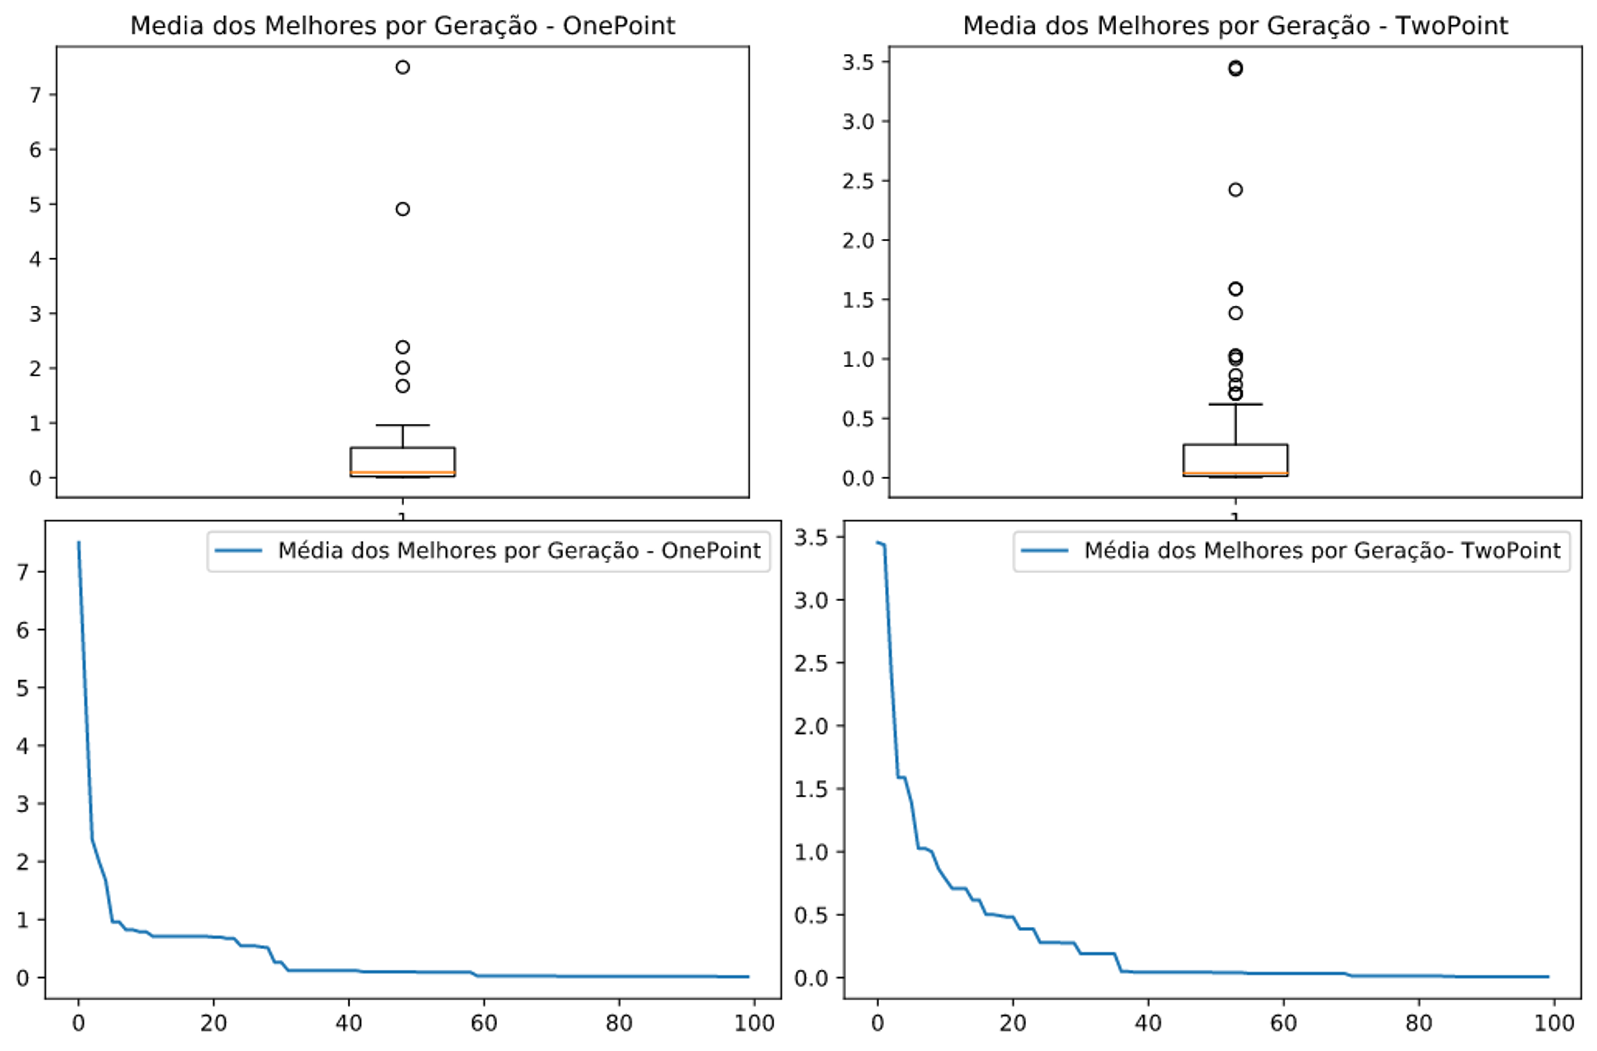
\includegraphics[width=0.9\linewidth]{Imagens/TipoCross}
		\caption{Variação crossover\_type}
		\label{fig:tipocross}
	\end{figure}
	
	Por fim, ao analisar os diferentes tipos de crossover, podemos observar que o uniforme é, conforme imaginado, o melhor. Isso se dá por ele ser capaz de realizar qualquer combinação entre os progenitores, garantindo maior variabilidade genética o que, principalmente junto com elitismo, favorece a evolução do GA. Nota-se que o boxplot do crossover uniforme possui segundo e terceiro quartis mais estreitos e próximos de zero do que os outros dois tipos. Além disso, o perfil descendente da curva de média dos melhores por geração também é mais acentuado.
	
	Sendo assim, dentre estes tipos clássico, o uniforme, para este problema, deve ser o escolhido.
	
	\section{GA com parâmetros escolhidos}
	
	Nesta seção será executado um GA com cada parâmetro do modelo igual ao melhor parâmetro de cada seção anterior. Isso será feito com o intuito principal de averiguar se a combinação dos melhores parâmetros escolhidos individualmente resulta em um melhor resultado quando comparado ao GA com os parâmetros default.
	
	A tabela abaixo exibe os parâmetros escolhidos:
	
	\begin{table}[H]
		\centering
		\begin{tabular}{|l|l|l|l|}
			\hline
			max\_num\_iterarion    & population\_size & mutation\_probability & elit\_ratio \\ \hline
			150                   & 250               & 0.3                    & 0.1           \\ \hline
			crossover\_probability & parents\_portion & crossover\_type       &             \\ \hline
			0.75                     & 0.3                & Uniform                     &             \\ \hline
		\end{tabular}
	\end{table}
	
	\begin{figure}[H]
		\centering
		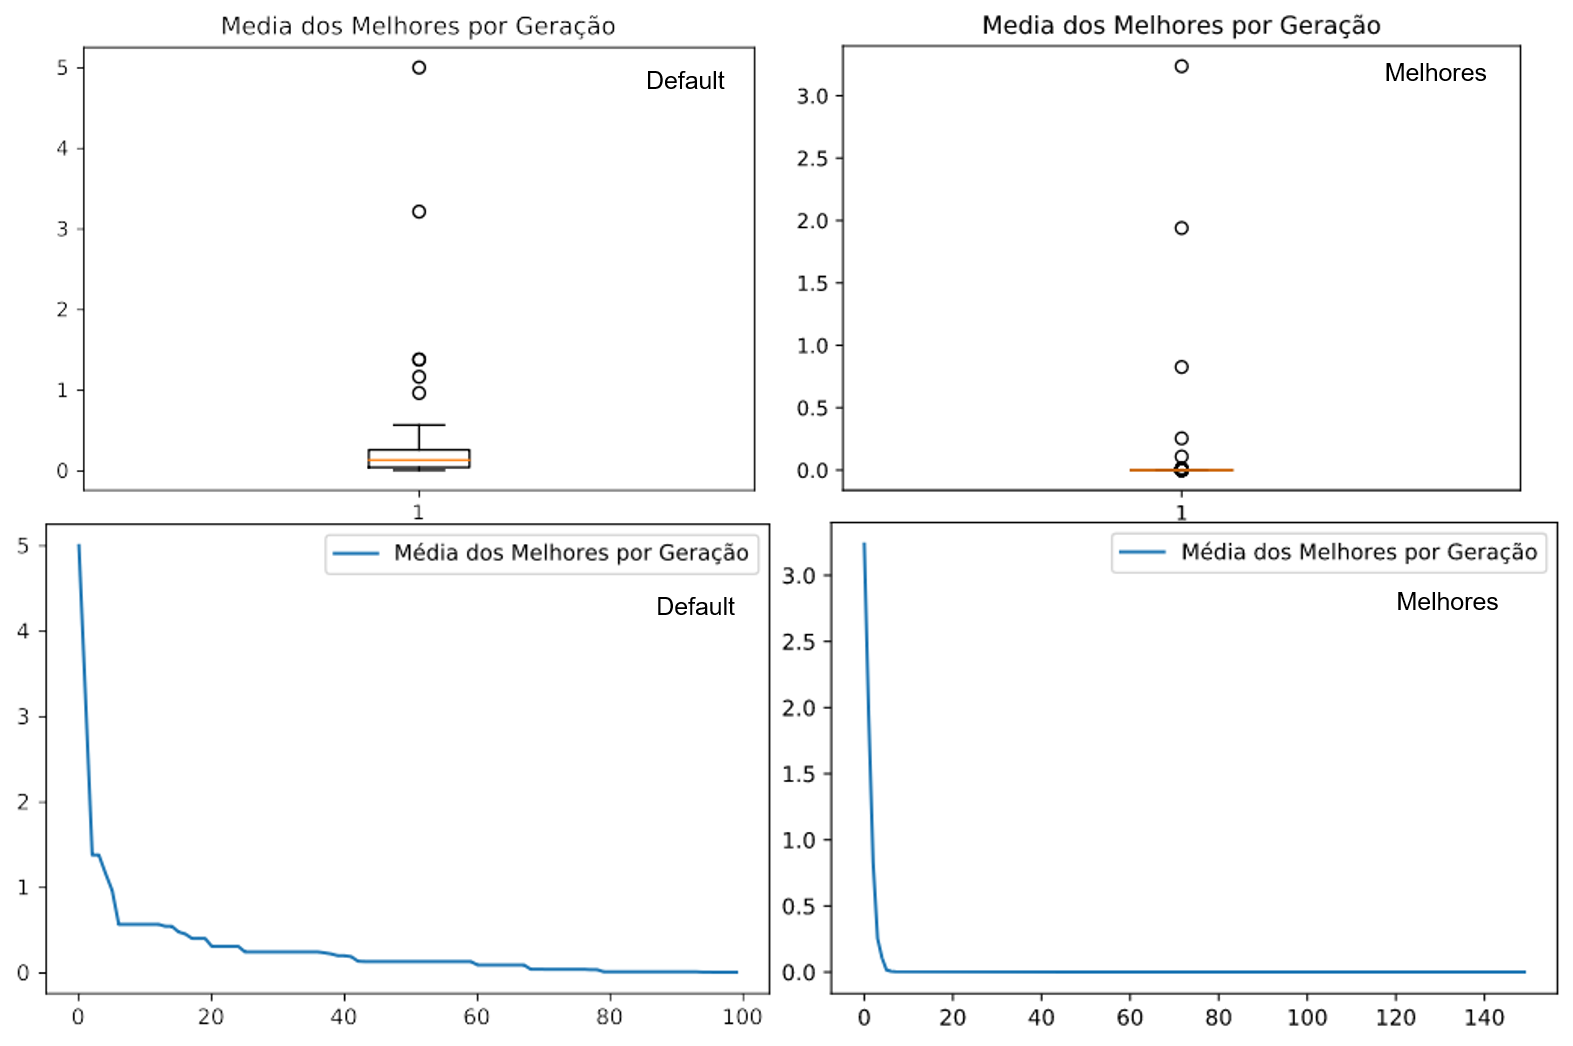
\includegraphics[width=0.9\linewidth]{Imagens/imagensMelhores}
		\caption{Boxplot e gráfico com parâmetros default e escolhidos}
		\label{fig:imagensmelhores}
	\end{figure}
	
	Como, nesta seção, variamos todos os parâmetros juntos, não podemos verificar o efeito de cada um separadamente assim como foi feito nas seções anteriores, mas podemos notar que a combinação de todos os valores escolhidos como os melhores valores para cada parâmetro gera um GA, para este problema, razoavelmente melhor que o GA com valores default. Isso é percebido tanto pelo perfil mais acentuado em direção ao valor mínimo quanto para a maior concentração de indivíduos próximo de zero, haja vista todos os quartis condensados nesse valor.
	
\end{document}